\documentclass{standalone}

\usepackage{amsmath}
\usepackage{tikz}
\usetikzlibrary{circuits.ee.IEC}
\usepackage{placeins}

\begin{document}
	
	
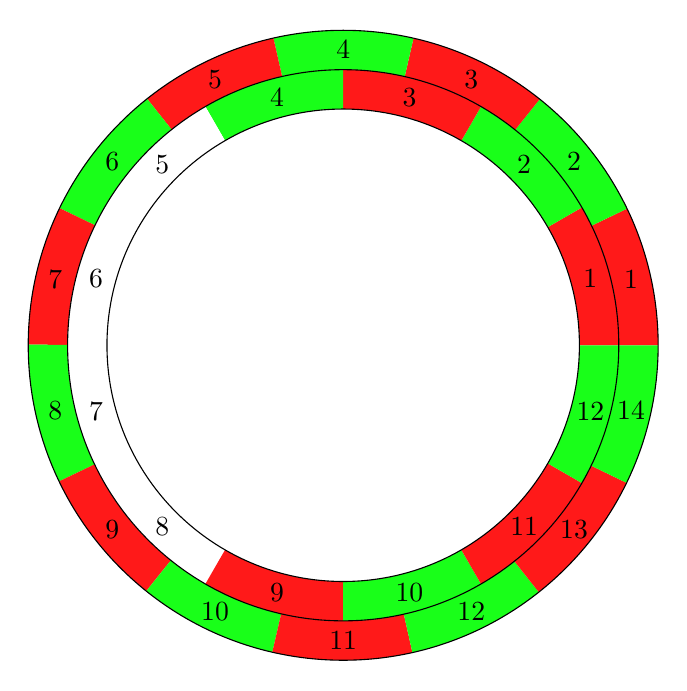
\begin{tikzpicture}[
		point/.style={circle,draw,minimum size=#1},
		point/.default=0pt]
		
		
		%rotor
		
		\foreach \anfang/\ende/\farbe in { 0/25.7/red!90, 25.7/51.4/green!90,  51.4/77.1/red!90, 77.1/102.8/green!90,  102.8/128.5/red!90, 128.5/154.2/green!90, 154.2/179.9/red!90, 
			179.9/205.6/green!90,  205.6/231.3/red!90, 231.3/257/green!90!,  257/282.7/red!90, 282.7/308.4/green!90,  308.4/334.1/red!90, 334.1/360/green!90}
		\draw[fill=\farbe,draw=none] (0,0) -- (\anfang:4cm) arc (\anfang:\ende:4cm);
		
		\draw[fill=white,draw=none] (0,0) circle (3.5cm);
		
		\foreach[count=\i,evaluate=\i as \angle using (\i-1)*(360/14)+12.85] \text in {1,2,3,4,5,6,7,8,9,10,11,12,13,14}
		\node (node\i) at (\angle:3.75) {\text};
		
		%stator
		\foreach \anfang/\ende/\farbe in { 0/30/red!90, 30/60/green!90,  60/90/red!90, 90/120/green!90,  120/150/white!90, 150/180/white!90, 
			180/210/white!90, 210/240/white!90,  240/270/red!90, 270/300/green!90!,  300/330/red!90, 330/360/green!90}
		\draw[fill=\farbe,draw=none] (0,0) -- (\anfang:3.5cm) arc (\anfang:\ende:3.5cm);
		
		\draw[fill=white,draw=none] (0,0) circle (3cm);
		
		\foreach[count=\i,evaluate=\i as \angle using (\i-1)*(360/12)+15] \text in {1,2,3,4,5,6,7,8,9,10,11,12}
		\node (node\i) at (\angle:3.25) {\text};
		
		%ränder	
		\draw (0,0) circle [radius=3cm];
		\draw (0,0) circle [radius=3.5cm];
		\draw (0,0) circle [radius=4cm];
		
		
		\end{tikzpicture}
		
		
\end{document}